% REVIEW DRAFT (2026-10-18) of the broadened summit poster. Not for print until collaborator approval.
% Numbers: records/CORA_SUMMIT_CLAIM_LEDGER_20261017.md. Figures: ../summit_poster/figures/ (PROVENANCE.json).
% Every number is indexed in records/CORA_SUMMIT_POSTER_EVIDENCE_20261012.md (section 15: the
% 14 October failure funnel and competition status, from records/CORA_FAILURE_FUNNEL_20261014.md).
% Every image is in figures/, drawn from hash-pinned recorded outputs by
% scripts/summit_figures.py at its printed size (9.50 in = one block's text
% width), with its provenance in figures/PROVENANCE.json. Diagrams are TikZ
% drawings of the real pipeline; dashed parts are proposed, not implemented.
% Type sizes: body 30 pt, secondary 26 pt, diagram and figure text >= 20 pt.
% Build: ./build.sh (reproducible: fixed SOURCE_DATE_EPOCH, no trailer id).
\RequirePackage{fix-cm}
\documentclass[25pt, a0paper, portrait]{tikzposter}
\usepackage[scaled]{helvet}
\renewcommand{\familydefault}{\sfdefault}
\usepackage[T1]{fontenc}
\usepackage{graphicx}
\usepackage{booktabs}
\usepackage{array}
\usepackage{enumitem}
\usetikzlibrary{positioning, arrows.meta, fit, calc}
\pdftrailerid{}

\newcommand{\bodyfont}{\fontsize{30}{37}\selectfont}
\newcommand{\secfont}{\fontsize{26}{32}\selectfont}
\newcommand{\diagfont}{\fontsize{25}{30}\selectfont}
\newcommand{\diagsub}{\fontsize{22}{27}\selectfont}
\newcommand{\questfont}{\fontsize{36}{44}\selectfont\bfseries}
\newcommand{\bt}[1]{{\fontsize{40}{48}\selectfont #1}}
\setlist{leftmargin=1.1em, itemsep=0.25em, topsep=0.3em, parsep=0pt}

\definecolor{ink}{HTML}{0B0B0B}
\definecolor{ink2}{HTML}{52514E}
\definecolor{accent}{HTML}{2A78D6}
\definecolor{warm}{HTML}{EB6834}
\definecolor{neutral}{HTML}{F0EFEC}
\definecolor{critical}{HTML}{D03B3B}
\definecolor{paper}{HTML}{FCFCFB}

\usetheme{Simple}
\tikzposterlatexaffectionproofoff
\colorlet{backgroundcolor}{paper}
\colorlet{framecolor}{paper}
\colorlet{titlefgcolor}{ink}
\colorlet{titlebgcolor}{paper}
\colorlet{blocktitlebgcolor}{paper}
\colorlet{blocktitlefgcolor}{accent}
\colorlet{blockbodybgcolor}{paper}
\colorlet{blockbodyfgcolor}{ink}
\makeatletter
\settitle{\centering\vbox{\color{titlefgcolor}{\bfseries\fontsize{84}{100}\selectfont \@title\par}\vspace*{0.45em}%
  {\fontsize{52}{62}\selectfont \@author\par}\vspace*{0.3em}{\fontsize{40}{48}\selectfont\color{ink2} \@institute}}}
\makeatother

\graphicspath{{../summit_poster/}}
\title{\parbox{0.94\linewidth}{\centering Learning What to Change: From Visual Reasoning\\ to Scientific Hypothesis Revision}}
\author{Chimdi Walter Ndubuisi \quad University of Missouri}
\institute{Executable reasoning, failure diagnosis and generalization across semantic domains \,$\cdot$\, {\color{critical}REVIEW DRAFT, 18 October}}

\tikzset{
  stage/.style={rounded corners=8pt, draw=accent, line width=2.2pt, fill=white, align=center,
                font=\diagfont, text width=20.4cm, inner sep=8pt},
  pstage/.style={stage, dashed, draw=ink2},
  choice/.style={rounded corners=8pt, draw=accent, line width=2pt, fill=white, align=center,
                 font=\diagfont, text width=6.1cm, minimum height=2.0cm, inner sep=6pt},
  pchoice/.style={choice, dashed, draw=ink2},
  flow/.style={-{Latex[length=7mm,width=5mm]}, line width=2.6pt, draw=ink2},
}

\begin{document}
\maketitle[width=0.97\linewidth]
\begin{columns}

%======================= COLUMN 1: the longstanding problem
\column{0.333}
\block{\bt{The question}}{\bodyfont
  How can a system learn to reason about things it was never explicitly programmed to understand? Three parts:
  \begin{enumerate}[leftmargin=1.3em]
    \item \textbf{Representation:} can it induce the right entities from sparse data of a new kind?
    \item \textbf{Rules:} can it discover the executable rules that act on them?
    \item \textbf{Revision and transfer:} when it fails, can it tell \emph{which part} to change, and does that
      procedure carry over to a domain whose meaning is different?
  \end{enumerate}
  \secfont These questions were shaped in discussion with Toni Kazic.
}
\block{\bt{Why one solved puzzle proves little}}{\bodyfont
  Several programs can fit every demonstration and still disagree on the test. On 60 exposed ARC-AGI-2
  training tasks, CORA's object reasoner had demonstration-fitting programs that were \textbf{all wrong} on
  26 tasks (with its frozen assets).
  \par\vspace{0.4em}
  A failure can come from three different places, and each needs a different change:
  \begin{itemize}
    \item the \textbf{representation} (which objects exist);
    \item the \textbf{rule} (what happens to them);
    \item the \textbf{evidence} (the examples do not decide).
  \end{itemize}
  The wrong revision can break what already worked.
}
\block{\bt{Where this sits}}{\bodyfont
  \begin{itemize}
    \item \textbf{Popper} (Cropper \& Morel): program induction that learns from failed hypotheses.
    \item \textbf{DreamCoder} (Ellis et al.), \textbf{LILO} (Grand et al.): growing reusable program libraries.
    \item \textbf{Model Discovery Agent} (Murphy): model inadequacy driving hypothesis revision and experiment design.
    \item Frontier neural reasoners are strong; they are comparisons, not straw men.
  \end{itemize}
  \secfont The narrower question here: choosing \emph{which component} to revise, and showing that this choice
  beats an equally equipped system that does not use the diagnosis.
}
\block{\bt{Four achievements, four statuses}}{\bodyfont\secfont
  \renewcommand{\arraystretch}{1.25}
  \begin{tabular}{@{}>{\raggedright\arraybackslash}p{0.56\linewidth}>{\raggedright\arraybackslash}p{0.40\linewidth}@{}}
  \toprule
  achievement & status \\ \midrule
  detect certain reasoning failures & built, with limits \\
  construct and verify an executable correction & shown: one synthetic task, one exposed real task \\
  learn to choose better revisions from failures & \textbf{not established} \\
  transfer a revision policy to biology & \textbf{not tested} \\ \bottomrule
  \end{tabular}
}
\block{\bt{The message}}{\bodyfont
  Intelligence may require more than finding an answer. It may require recognizing when the concepts and
  rules used to build the answer are inadequate, and deciding what must change.
}

%======================= COLUMN 2: what CORA has measured
\column{0.333}
\block{\bt{Where CORA fails on real tasks \;{\color{warm}DONE}}}{\bodyfont
  \begin{tikzfigure}
    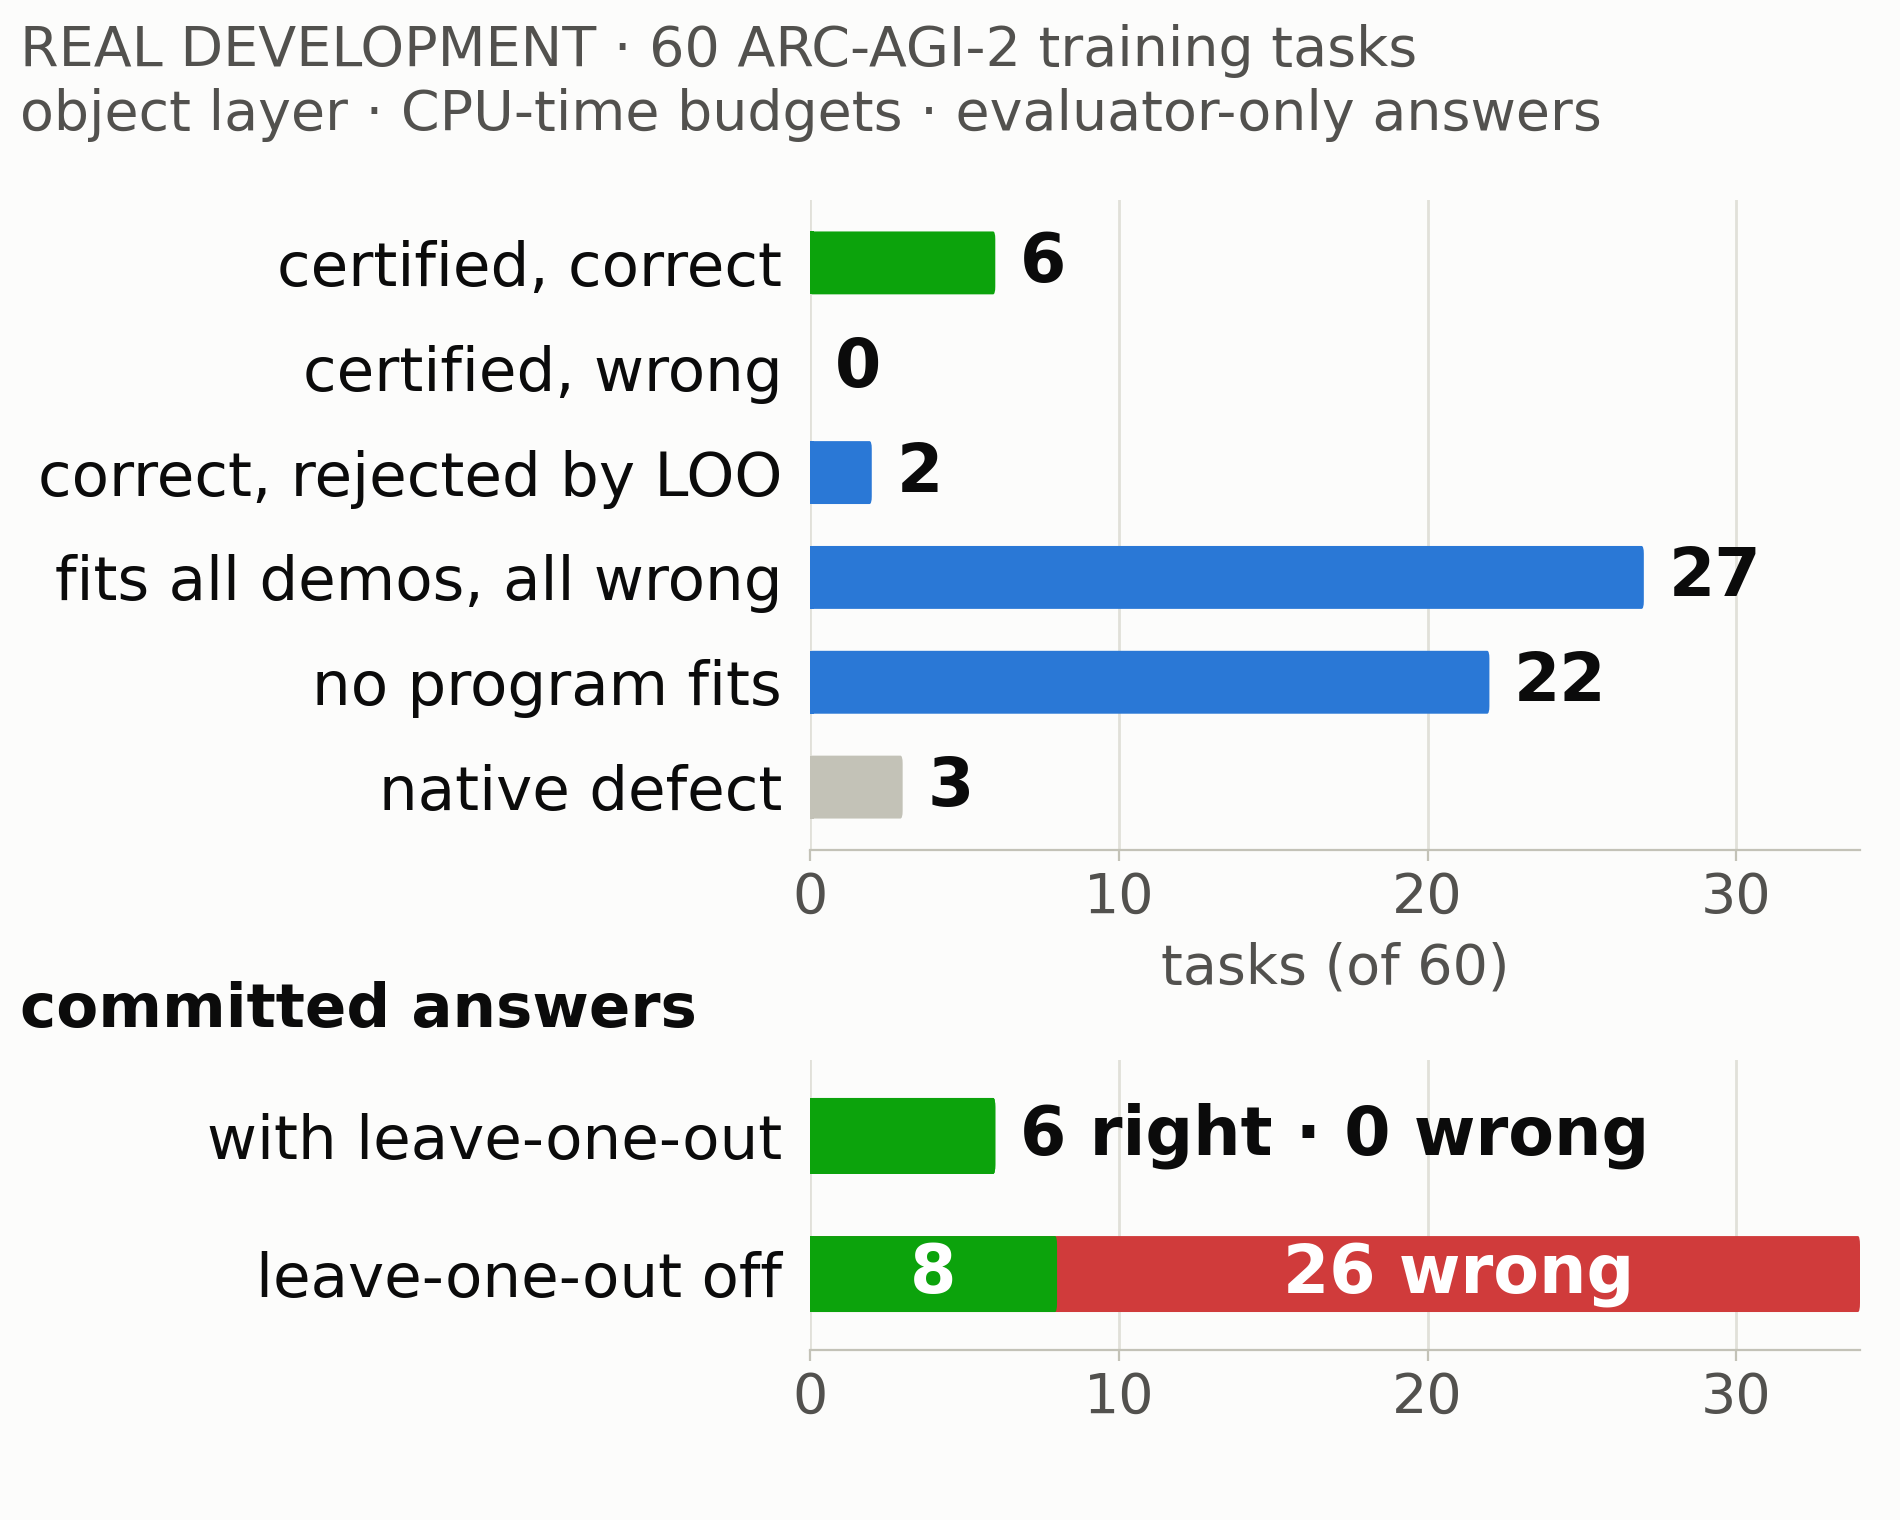
\includegraphics[width=\linewidth]{figures/fig_failure_funnel_dev60.png}
  \end{tikzfigure}
  \secfont Object reasoner, 60 exposed training tasks. Figure: run without the frozen assets (27
  all-wrong fits; check off, 8 right and 26 wrong). As submitted, with the assets: 26, and 8 right and 25
  wrong. In both, the check accepted 6 answers, all correct, and a correct candidate existed on 8. This is
  one branch, not a reliable solver.
}
\block{\bt{Building a missing rule, verified \;{\color{warm}DONE, NARROW}}}{\bodyfont
  \begin{tikzfigure}
    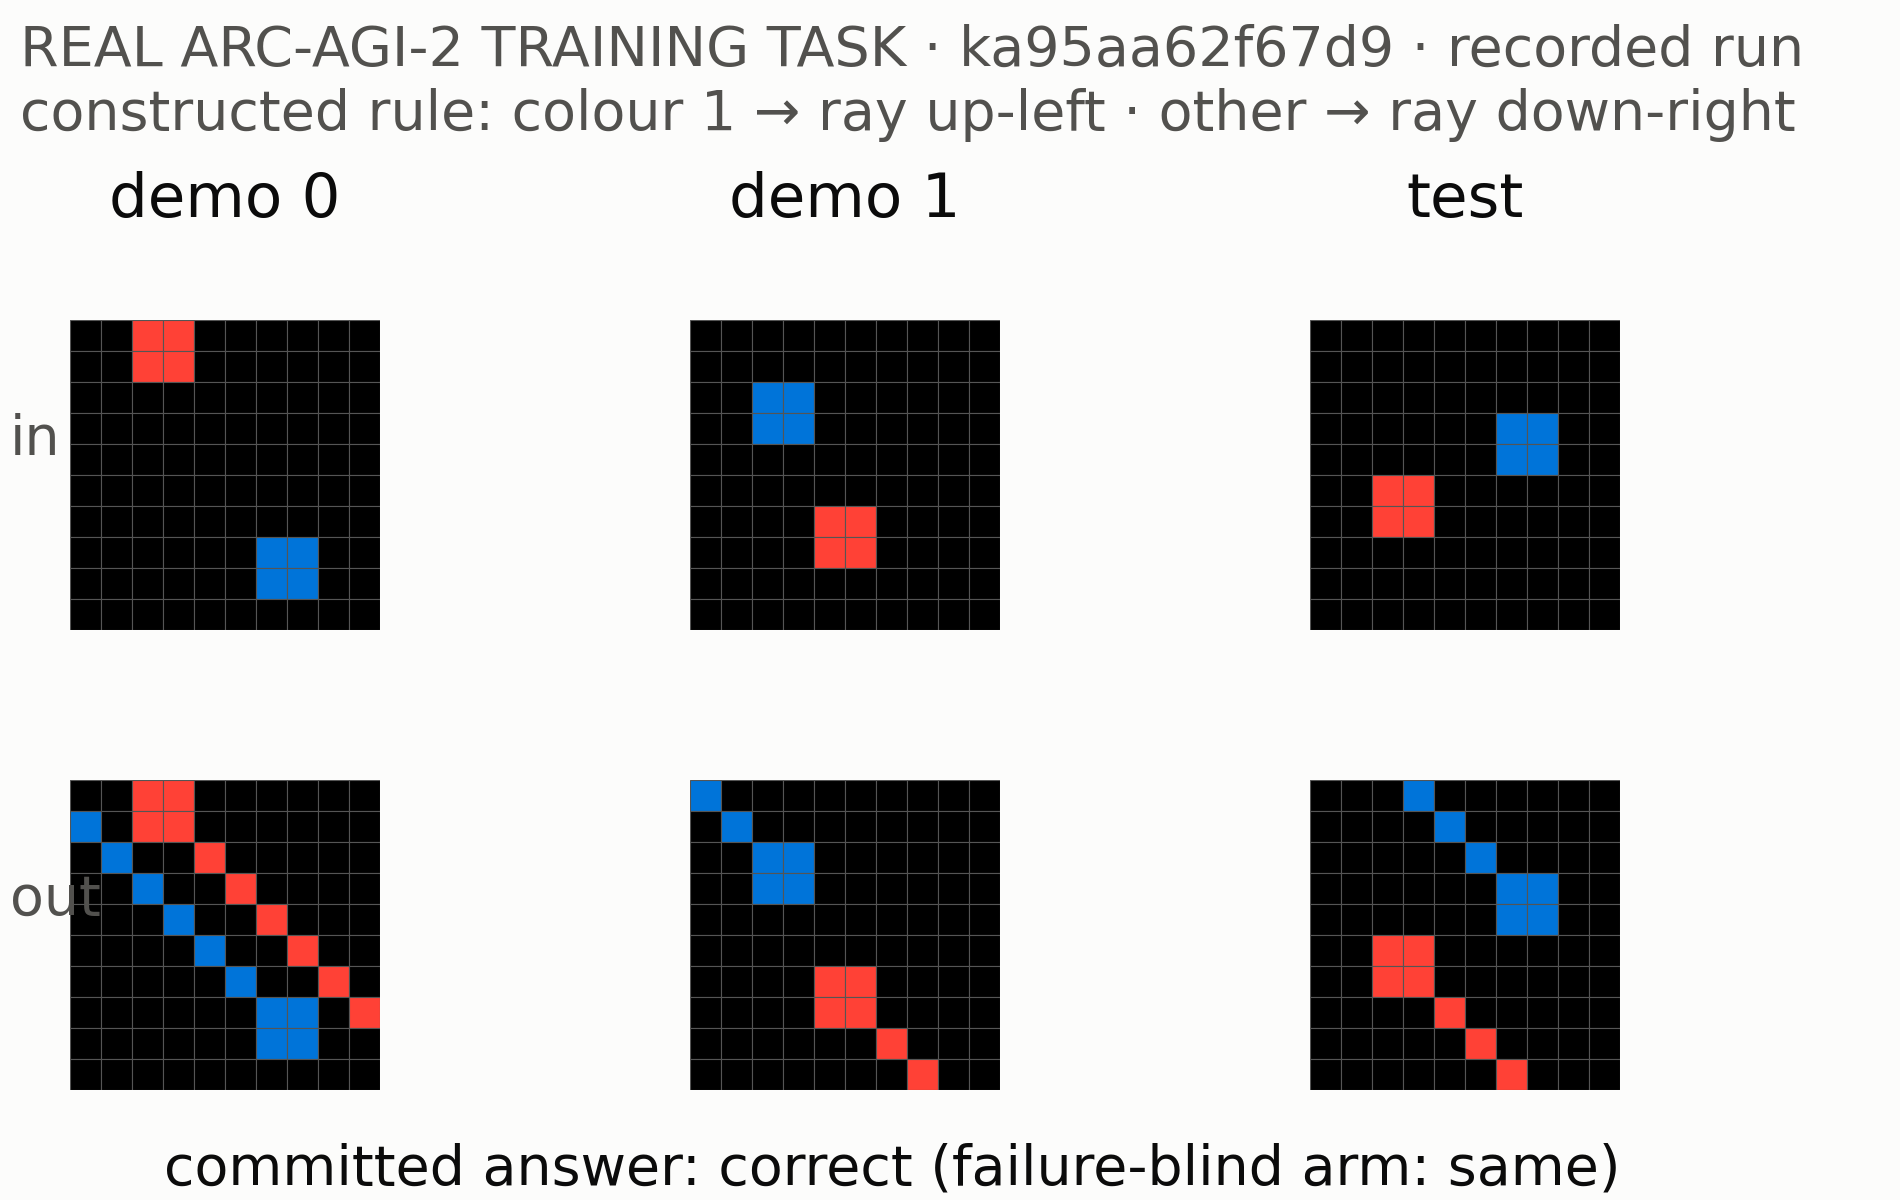
\includegraphics[width=\linewidth]{figures/fig_fhr_real_witness_ka95aa62f67d9.png}
  \end{tikzfigure}
  \secfont \textbf{Real training task.} Frozen CORA and extra search both fail. CORA built a rule that says
  \emph{where} it applies as well as \emph{what} it does: colour-1 objects shoot a ray north-west, others
  south-east. It was installed reversibly, rebuilt in 3 of 3 leave-one-out folds, and answered correctly.
  \textbf{Limits:} the failure autopsy selected the task; it is an exposed training task; a failure-blind
  constructor found the same rule.
  \par\vspace{0.3em}
  \textbf{Synthetic task:} a single-step ring around the minority-colour cell, 3 of 3 folds, correct.
}
\block{\bt{Does learning from the failure help? \;{\color{critical}NOT ESTABLISHED}}}{\bodyfont\secfont
  \begin{itemize}
    \item A frozen 10-case pilot: failure record 2 correct, failure-blind 1 correct plus 1 tie abstention,
      0 wrong, 0 lost. One discordant pair ($p = 0.5$) is not evidence.
    \item A hand-designed controller that picks the kind of revision missed the only task that extra search
      fixed: 6 against 7.
    \item Why construction rarely fires: of 62 eligible tasks, 20 left no evidence and 39 had evidence no rule
      fitted. Of 25 such real cases, 18 were inexpressible in the grammar.
  \end{itemize}
  \bodyfont\textbf{Constructing a rule and learning which revision to make are different capabilities.}
}

%======================= COLUMN 3: from ARC to scientific discovery
\column{0.333}
\block{\bt{A revision architecture \;{\color{ink2}solid: built \,$\cdot$\, dashed: proposed}}}{\bodyfont
  \begin{tikzfigure}
  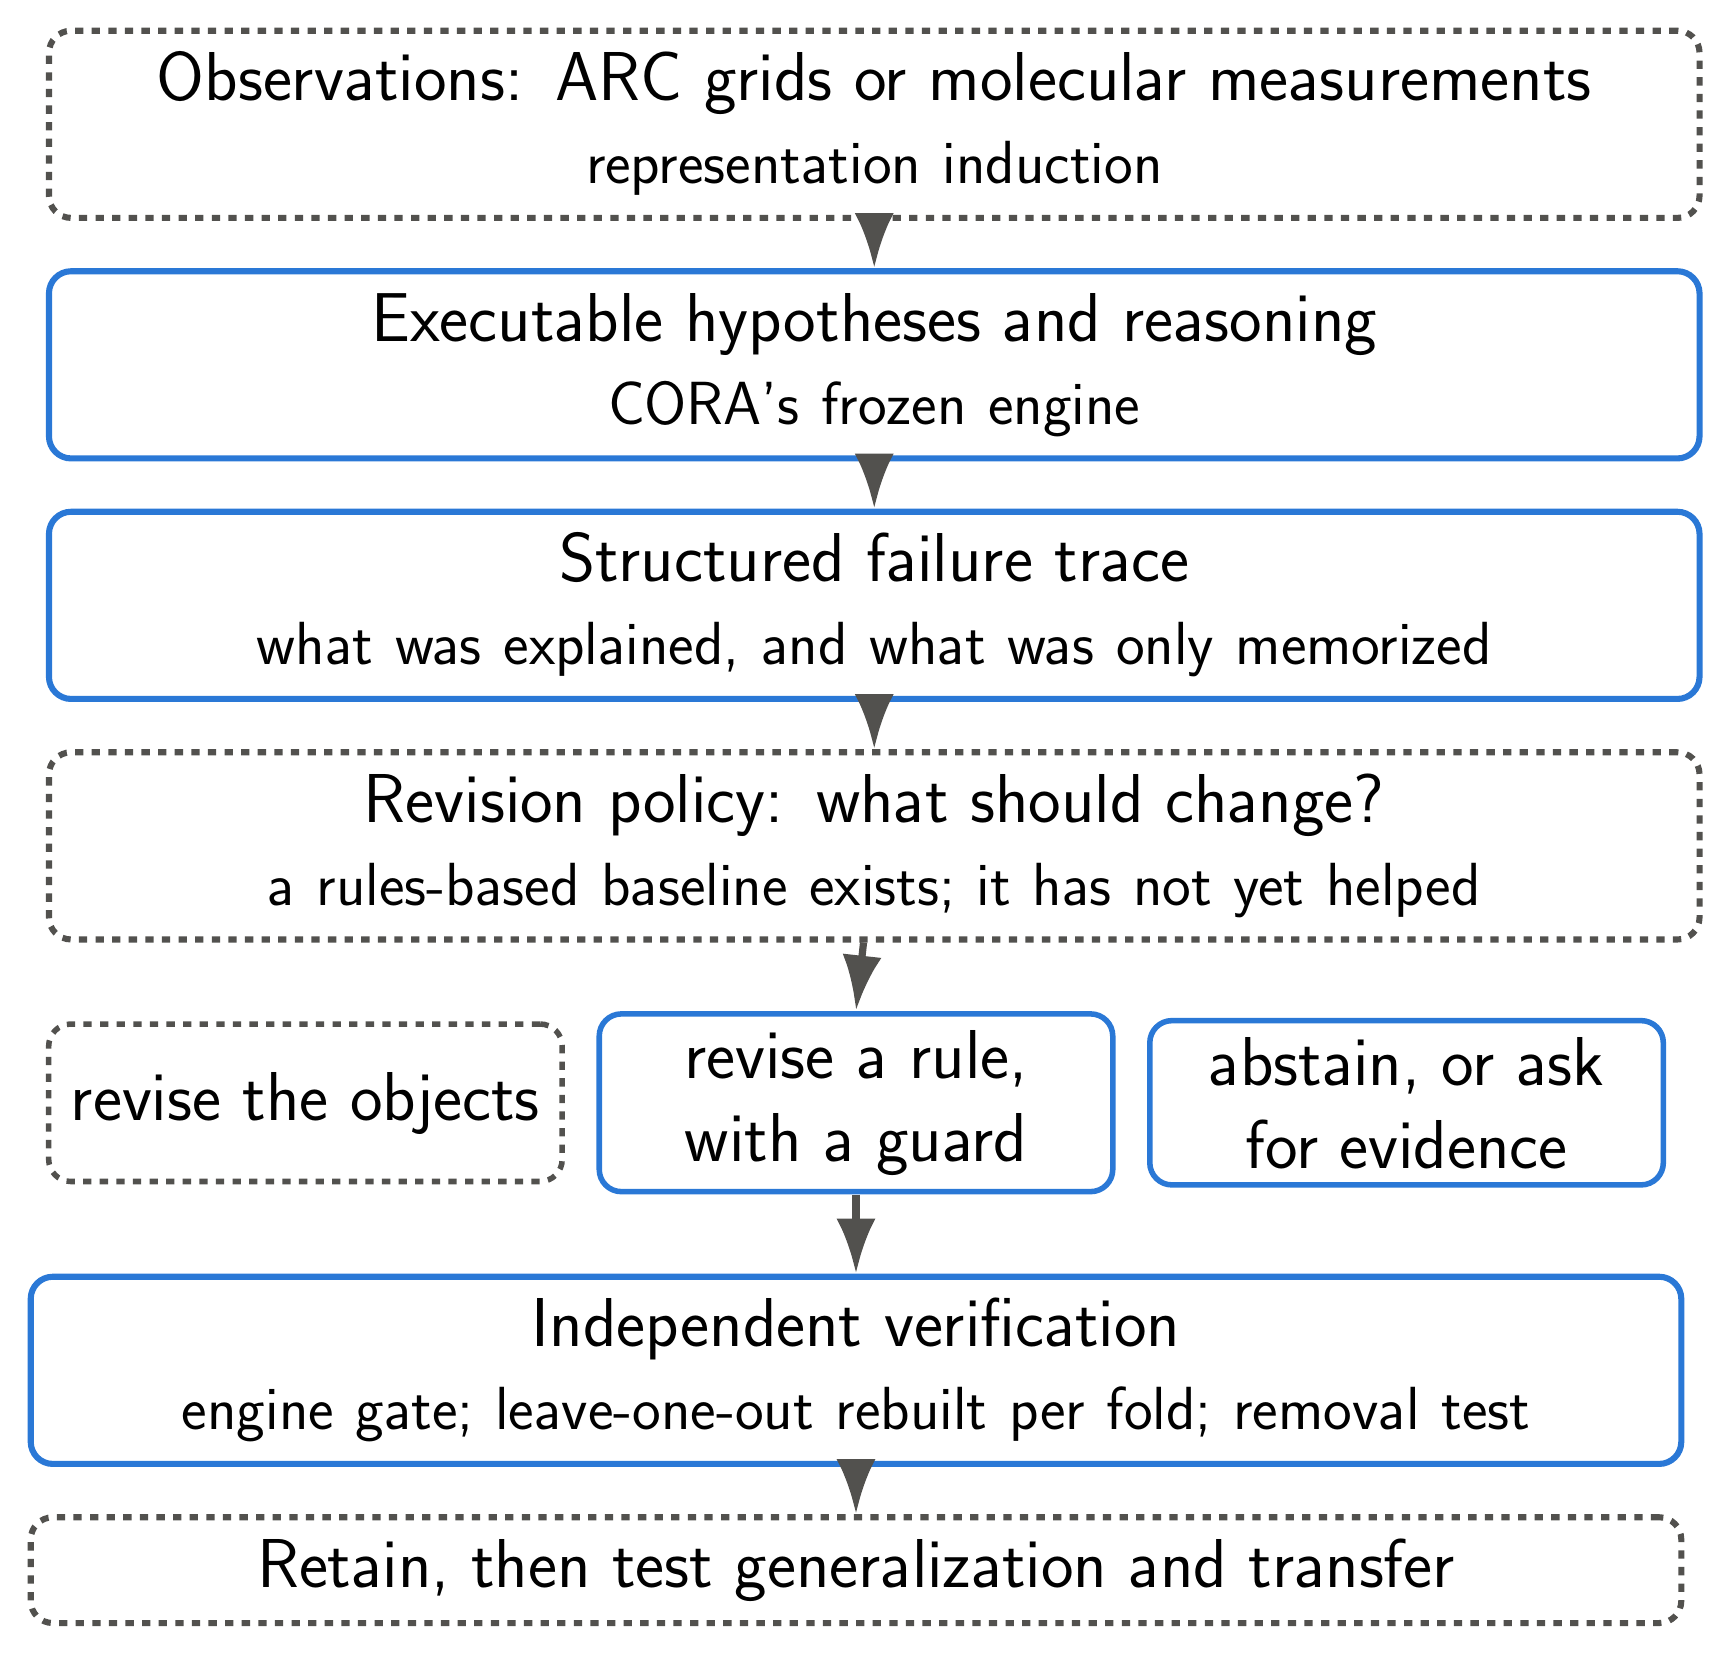
\begin{tikzpicture}[node distance=0.6cm]
    \node[pstage] (o) {Observations: ARC grids or molecular measurements\\ \diagsub representation induction};
    \node[stage, below=of o] (h) {Executable hypotheses and reasoning\\ \diagsub CORA's frozen engine};
    \node[stage, below=of h] (t) {Structured failure trace\\ \diagsub what was explained, and what was only memorized};
    \node[pstage, below=of t] (p) {Revision policy: what should change?\\ \diagsub a rules-based baseline exists; it has not yet helped};
    \node[pchoice, below=1.0cm of p.south west, anchor=north west] (r1) {revise the objects};
    \node[choice, right=0.4cm of r1] (r2) {revise a rule, with a guard};
    \node[choice, right=0.4cm of r2] (r3) {abstain, or ask for evidence};
    \node[fit=(r1)(r2)(r3), inner sep=0pt] (g) {};
    \node[stage, below=1.0cm of g] (v) {Independent verification\\ \diagsub engine gate; leave-one-out rebuilt per fold; removal test};
    \node[pstage, below=of v] (x) {Retain, then test generalization and transfer};
    \draw[flow] (o) -- (h); \draw[flow] (h) -- (t); \draw[flow] (t) -- (p);
    \draw[flow] (p) -- (g.north); \draw[flow] (g.south) -- (v); \draw[flow] (v) -- (x);
  \end{tikzpicture}
  \end{tikzfigure}
}
\block{\bt{The next falsifiable test \;{\color{ink2}RUNNING}}}{\bodyfont\secfont
  58 independently selected training tasks, frozen before the run. It asks whether failure information
  chooses better revisions than an equally equipped failure-blind constructor. One new arm learns
  \emph{what} to change from what the solver could only memorize, and \emph{where} from the boundary with
  what it explains. Paired sign tests, Holm-corrected; results will be reported only after validation.
}
\block{\bt{Scientific prediction \;{\color{critical}PROPOSED, NOT TESTED}}}{\bodyfont\secfont
  With molecular measurements, should the system revise its representation, revise its hypothesis, or ask
  for an experiment? What could transfer is the revision policy and the verification interface, not ARC
  operators. A biological check needs tolerance, real replicates, held-out conditions and experiments, not
  exact match. The problem contract (questions for Pierce and Toni) is in review; no biological result is
  claimed.
}
\block{\bt{Benchmark context}}{\bodyfont\secfont
  Official ARC-AGI-2 public scores: native CORA \textbf{0.00}; a reproduction of the published NVARC
  Qwen3-4B pipeline \textbf{27.64}, which is \textbf{not CORA}. The CORA-FHR research entry (18 October) scored
  \textbf{0.00}, as its local rehearsal predicted (no new answer committed). The guarded rule came
  later and is not part of it.
}
\block{\bt{The question I want to pursue}}{\bodyfont
  Can a reasoning system learn from the boundary between what its current knowledge explains and what it
  cannot, decide what must change, and acquire a capability that generalizes? ARC offers a controlled place
  to find out before testing it in science.
  \par\vspace{0.3em}{\raggedright\diagsub Every number, with its scope and hash:
  \texttt{records/CORA\_SUMMIT\_CLAIM\_LEDGER\_20261017.md}. Authorship and credits are pending collaborator
  review.\par}
}
\end{columns}
\end{document}
